% Created 2018-04-09 Mon 16:13
% Intended LaTeX compiler: pdflatex
\documentclass[10pt]{beamer}
\usepackage[utf8]{inputenc}
\usepackage[T1]{fontenc}
\usepackage{graphicx}
\usepackage{grffile}
\usepackage{longtable}
\usepackage{wrapfig}
\usepackage{rotating}
\usepackage[normalem]{ulem}
\usepackage{amsmath}
\usepackage{textcomp}
\usepackage{amssymb}
\usepackage{capt-of}
\usepackage{hyperref}
\usetheme{Boadilla}
\author{ECON 499: Growth and Development}
\date{Spring 2018}
\title{Introduction}
\usecolortheme{seagull}
\usefonttheme[onlylarge]{structurebold}
\usefonttheme[onlymath]{serif}
\setbeamerfont*{frametitle}{size=\normalsize,series=\bfseries}
\setbeamertemplate{navigation symbols}{}
\setbeamertemplate{itemize item}[triangle]
\setbeamertemplate{footline}{}
\setbeamertemplate{enumerate items}[default]
\hypersetup{
 pdfauthor={ECON 499: Growth and Development},
 pdftitle={Introduction},
 pdfkeywords={},
 pdfsubject={},
 pdfcreator={Emacs 25.2.2 (Org mode 9.1.6)}, 
 pdflang={English}}
\begin{document}

\maketitle

\begin{frame}[label={sec:org10367d4}]{}
\alert{Instructor}
\begin{itemize}
\item Michael Jerman (call me Michael)
\item Office: 342 Bexell
\item Email: michael.jerman@oregonstate.edu
\item Office hours:
\begin{itemize}
\item M/W: 10:30am-11:30am
\item T/Th: 8:30am-9:30am
\end{itemize}
\end{itemize}
\end{frame}

\begin{frame}[label={sec:orga496316}]{}
\alert{Prerequisites}
\begin{itemize}
\item Econ 311 (intermediate micro)
\item Econ 320 (intermediate macro)
\end{itemize}
\end{frame}

\begin{frame}[label={sec:org5b6b125}]{}
\alert{Textbook}
\begin{itemize}
\item \emph{Economic Growth}, Weil
\begin{itemize}
\item 3rd edition
\end{itemize}
\item \href{https://www.amazon.com/Economic-Growth-3rd-David-Weil/dp/0321795733/}{Amazon}
\begin{itemize}
\item \$108 new
\item \$34 used
\item \$15 rent (electronic version)
\end{itemize}
\item \href{http://verbacompare.osubeaverstore.com/comparison?id=2018-Spring\_\_ECON\_\_499\_\_002}{Bookstore}
\begin{itemize}
\item \$166 new
\item \$125 used
\end{itemize}
\item \href{https://www.abebooks.com/servlet/SearchResults?isbn=0321795733\&sts=t}{ABE Books}
\begin{itemize}
\item \$20 (international version)
\end{itemize}
\end{itemize}
\end{frame}

\begin{frame}[label={sec:orgdd36081}]{}
\alert{Canvas}
\begin{itemize}
\item Official course website
\item You are responsible for any and all information posted to Canvas
\item Contact canvas@oregonstate.edu if you have any issues
\end{itemize}
\end{frame}

\begin{frame}[label={sec:org9c8c708}]{}
\alert{Homework}
\begin{itemize}
\item Four graded homework assignments, posted on Canvas
\item Mix of problems from the text and other problems
\item Work in groups!
\begin{itemize}
\item Each person must submit their own assignment
\end{itemize}
\item Graded primarily on effort and completion
\begin{itemize}
\item 30\% of your grade just for doing the homework!
\end{itemize}
\end{itemize}
\end{frame}

\begin{frame}[label={sec:orgb5bd326}]{}
\alert{Exams}
\begin{itemize}
\item Midterm: Thursday, May 8 
\begin{itemize}
\item Week 6
\end{itemize}
\item Final: Tuesday, June 12 at 9:30am 
\begin{itemize}
\item Note that the university might change the final exam date
\end{itemize}
\item No makeup exams (see syllabus)
\end{itemize}
\end{frame}

\begin{frame}[label={sec:org06fc7f1}]{}
\alert{Grade}
\begin{center}
\begin{tabular}{ll}
Homework & 30\%\\
Midterm & 30\%\\
Final & 40\%\\
\end{tabular}
\end{center}
\end{frame}

\begin{frame}[label={sec:org20b5cec}]{}
\alert{Student conduct}
\begin{itemize}
\item Student's are bound by the university's \href{http://studentlife.oregonstate.edu/sites/studentlife.oregonstate.edu/files/code\_of\_student\_conduct.pdf}{Code of Student Conduct}
\item Any incidence of academic misconduct will result in a grade of "F" for the course 
\begin{itemize}
\item Additional sanctions may be imposed by the university
\end{itemize}
\end{itemize}
\end{frame}

\begin{frame}[label={sec:org95d9c05}]{}
\alert{Important dates}
(Subject to change)
\begin{center}
\begin{tabular}{ll}
Thursday, April 19 & Homework 1\\
Thursday, May 3 & Homework 2\\
Tuesday, May 8 & Midterm\\
Thursday, May 24 & Homework 3\\
Thursday, June 7 & Homework 4\\
Tuesday, June 12 & Final exam\\
\end{tabular}
\end{center}
\end{frame}

\begin{frame}[label={sec:orgc10eee4}]{}
\alert{Reading}
\begin{itemize}
\item This week: Chapters 1 \& 2
\item Next week: Chapter 3
\end{itemize}
\end{frame}

\begin{frame}[label={sec:org150aa49}]{}
\alert{Homework problems}
\begin{itemize}
\item Chapter 1 (page 24): 3, 5, 6
\item Chapter 2 (pages 46-47): 4, 5
\end{itemize}
\end{frame}

\begin{frame}[label={sec:org5ab500e}]{}
\alert{Some facts}
\begin{itemize}
\item 7.5 billion people alive
\item 925 million (12\%) people do not get enough food
\item 824 million (11\%) do not have access to clean water
\item 2.5 billion (33\%) lack sanitation
\item 2.6 billion (35\%) earn less than \$2 per day
\end{itemize}
\end{frame}

\begin{frame}[label={sec:orga757789}]{}
\alert{Cross-country differences}
\begin{itemize}
\item The people that live in the richest 20\% of countries earns 60\% of world income
\item Australia has 687 automobiles per 1000 people, Bangladesh has 2
\end{itemize}
\end{frame}

\begin{frame}[label={sec:orgc8c300f}]{}
\alert{Differences over time}
\begin{itemize}
\item A Japanese baby born in 1880 could expect to live 35 years
\item A Japanese baby born today can expect 83 years
\item Americans spend 3 times as much on recreation as a hundred years ago (as fraction of total income), 1/3 as much on food
\item Average workweek in 1870: 63 hours; today 34 hours
\item 200 million fewer Chinese people earn less than \$2 per day than they did 30 years ago
\end{itemize}
\end{frame}

\begin{frame}[label={sec:org06200c4}]{}
\alert{Income and GDP}
\begin{itemize}
\item Income is a good, but imperfect measure of well-being
\item We can usually measure income across countries (GDP)
\item Differences in income are vast, useful for understanding broad patterns in well-being
\end{itemize}
\end{frame}

\begin{frame}[label={sec:orgeee0217}]{}
\alert{Real vs nominal GDP}
\begin{itemize}
\item Nominal GDP is the price of all final goods and services produced within a country in a single year
\item Equal to total income (everything that is bought is also sold)
\item Price levels change: if all prices increase but we are not producing any more goods and services, nominal GDP will still increase
\item Solution: use prices from the same year (2005)
\item The \alert{\alert{2005 price}} of all goods and services produced within a country in a single year is \emph{real GDP}
\end{itemize}
\end{frame}

\begin{frame}[label={sec:org22cb917}]{}
\alert{Purchasing power parity (PPP)}
\begin{itemize}
\item Prices in each country are denominated in local currencies
\item Prices vary greatly across countries
\item Solution: calculate the price of a common "basket" of goods in each country, use that price to convert GDP to a common currency (usually 2005 USD)
\item In this class we will almost always use PPP adjusted real GDP numbers
\end{itemize}
\end{frame}

\begin{frame}[label={sec:org1ff3971}]{}
\alert{Pen's parade of global income}
\begin{itemize}
\item Suppose we split national income equally among all inhabitants of each country, each person has the national average income (per capita GDP)
\item Next suppose each person's height is proportional to their income, with average global income being an average height (6ft)
\item Now sit in one place and watch the entire world march by in a parade lasting one hour
\end{itemize}
\end{frame}

\begin{frame}[label={sec:org97c826c}]{}
\alert{First 7 minutes:}
\begin{itemize}
\item Mostly Sub-Saharan Africans, height less than 1 foot.
\end{itemize}
\end{frame}

\begin{frame}[label={sec:orgc450555}]{}
\alert{India and China:}
\begin{itemize}
\item India begins walking by in the 13 minute, lasting 11 minutes
\item Marchers are 23 inches tall
\item China begins around 30 minutes (half-way)
\item Marchers are 55 inches tall
\end{itemize}
\end{frame}

\begin{frame}[label={sec:orgf8268b0}]{}
\alert{Average height (income)}
\begin{itemize}
\item People with the average height start walking by around 45 minutes, after 3/4 of the world has walked by
\end{itemize}
\end{frame}

\begin{frame}[label={sec:orgaff39bc}]{}
\alert{The giants}
\begin{itemize}
\item 50 minute marchers are 9ft tall (Croatia)
\item 52 minute marchers are 18ft tall (Japan)
\item 55 minute marchers are 25ft tall (US)
\item The last 15 seconds: Marchers range from 32ft to 95ft tall
\end{itemize}
\end{frame}

\begin{frame}[label={sec:org5036c4a}]{}
\begin{center}
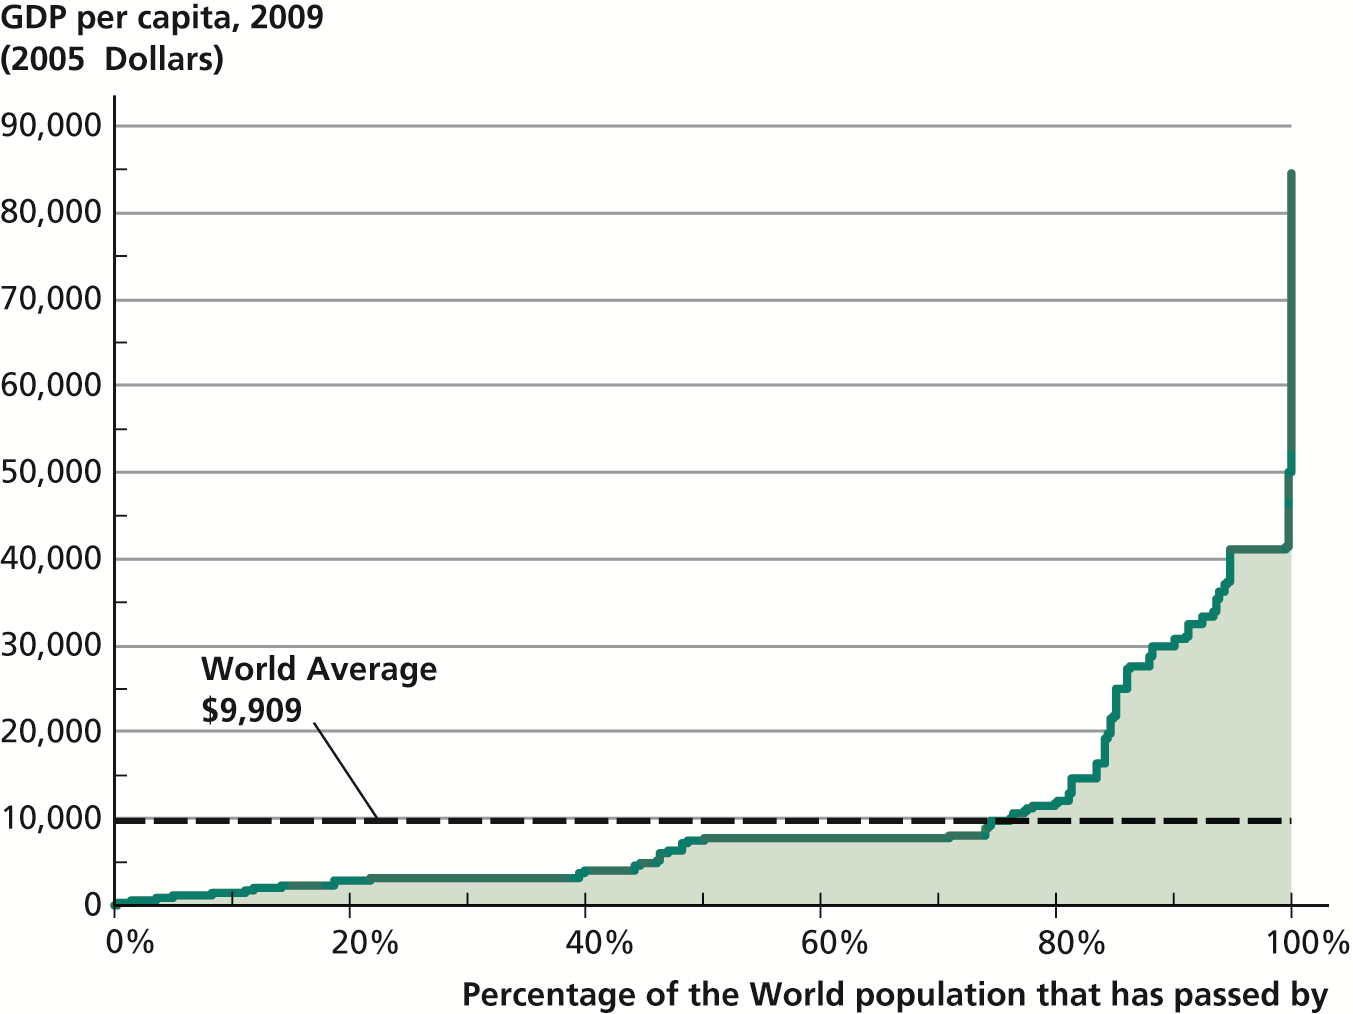
\includegraphics[width=.75\textwidth]{./img/1.1.png}
\end{center}
\end{frame}


\begin{frame}[label={sec:orgf268b9a}]{}
\alert{Growth}
\begin{itemize}
\item A "rate of growth" is the \emph{proportional} change in a series over some length of time
\item We will usually consider annual growth rates -- the rate of change over a year
\item Example: China's growth rate of GDP was 6.7\% in 2006. This means that China's GDP was 6.7\% larger in 2006 than it was in 2005
\end{itemize}
\end{frame}

\begin{frame}[label={sec:org8696d45}]{}
\alert{Growth and levels}
\begin{itemize}
\item A constant growth rate means that a series is growing \emph{exponentially}
\item It is common to express exponential growth using a "ratio" (or "logarithmic") scale
\end{itemize}
\end{frame}

\begin{frame}[label={sec:org1656461}]{}
\begin{center}
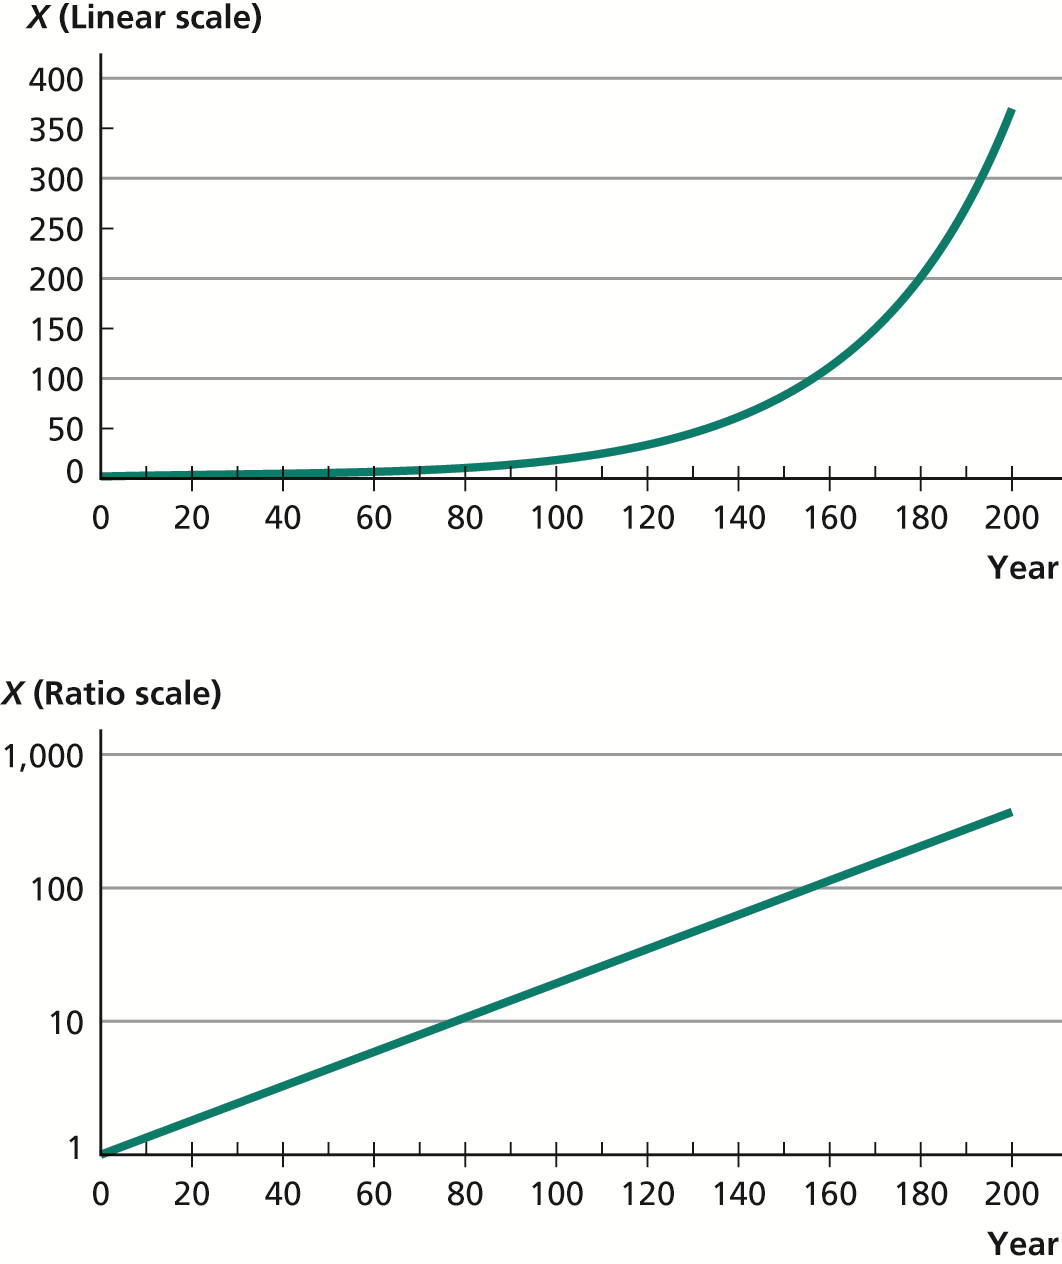
\includegraphics[height=.9\textheight]{./img/1.3.png}
\end{center}
\end{frame}

\begin{frame}[label={sec:orgb4dbdcc}]{}
\begin{center}
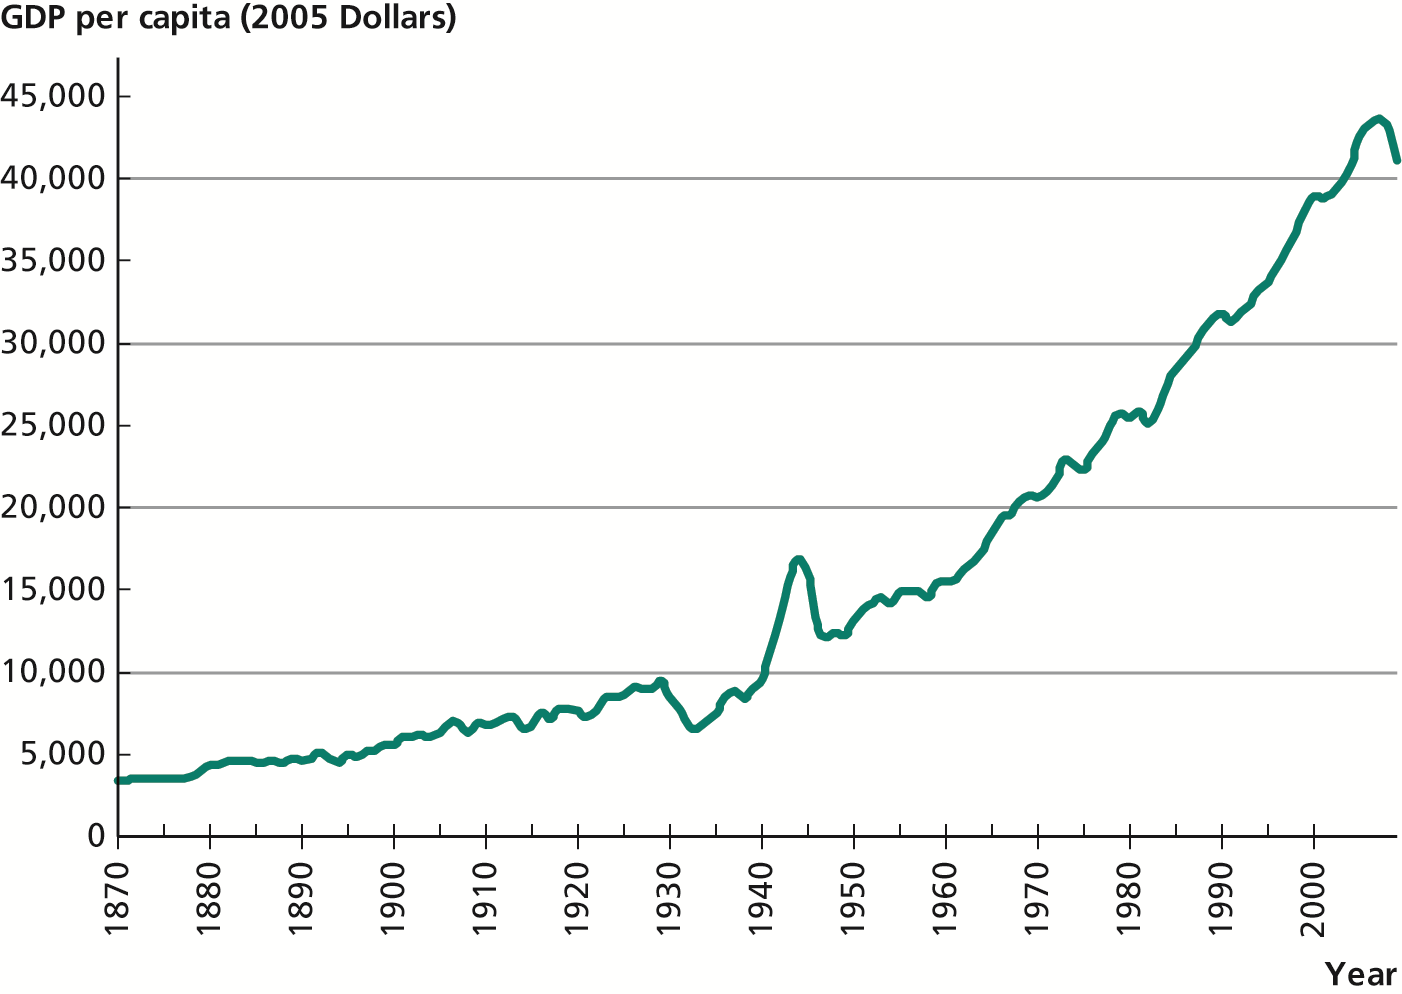
\includegraphics[width=.75\textwidth]{./img/1.2.png}
\end{center}
\end{frame}

\begin{frame}[label={sec:org15fc9f3}]{}
\begin{center}
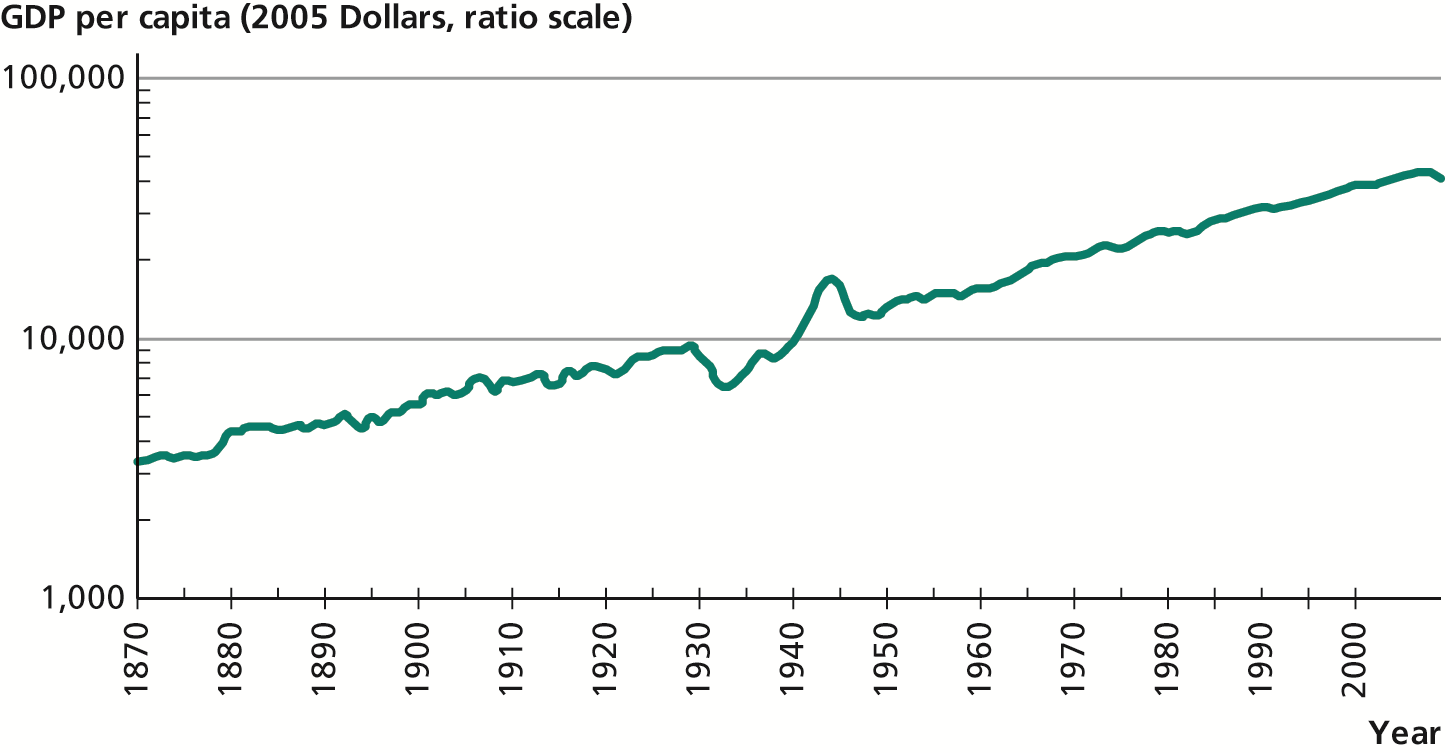
\includegraphics[width=.75\textwidth]{./img/1.4.png}
\end{center}
\end{frame}

\begin{frame}[label={sec:org926642a}]{}
\alert{Rule of 72}
\begin{itemize}
\item If a series grows at a rate g per year, the series will double in size every \(\frac{72}{100*g}\) years \(\left(\frac{72}{g\%}\right)\)
\item Example: Suppose Chinese GDP grows at 6\% every year. Then GDP will double in \(\frac{72}{100*0.06} = 12\) years
\end{itemize}
\end{frame}

\begin{frame}[label={sec:org371f87f}]{}
\alert{Growth across countries}
\begin{itemize}
\item The US shows remarkably constant growth historically
\item In general, it is not the case that countries have constant growth
\item The "rule of 72" shows how small differences in growth can translate into vastly different living standards
\item Since 1870, US grew at an average of 1.8\%, UK by 1.5\%
\item UK was 31\% richer in 1870, 19\% poorer today (per capita)
\end{itemize}
\end{frame}

\begin{frame}[label={sec:org5bfe483}]{}
\begin{center}
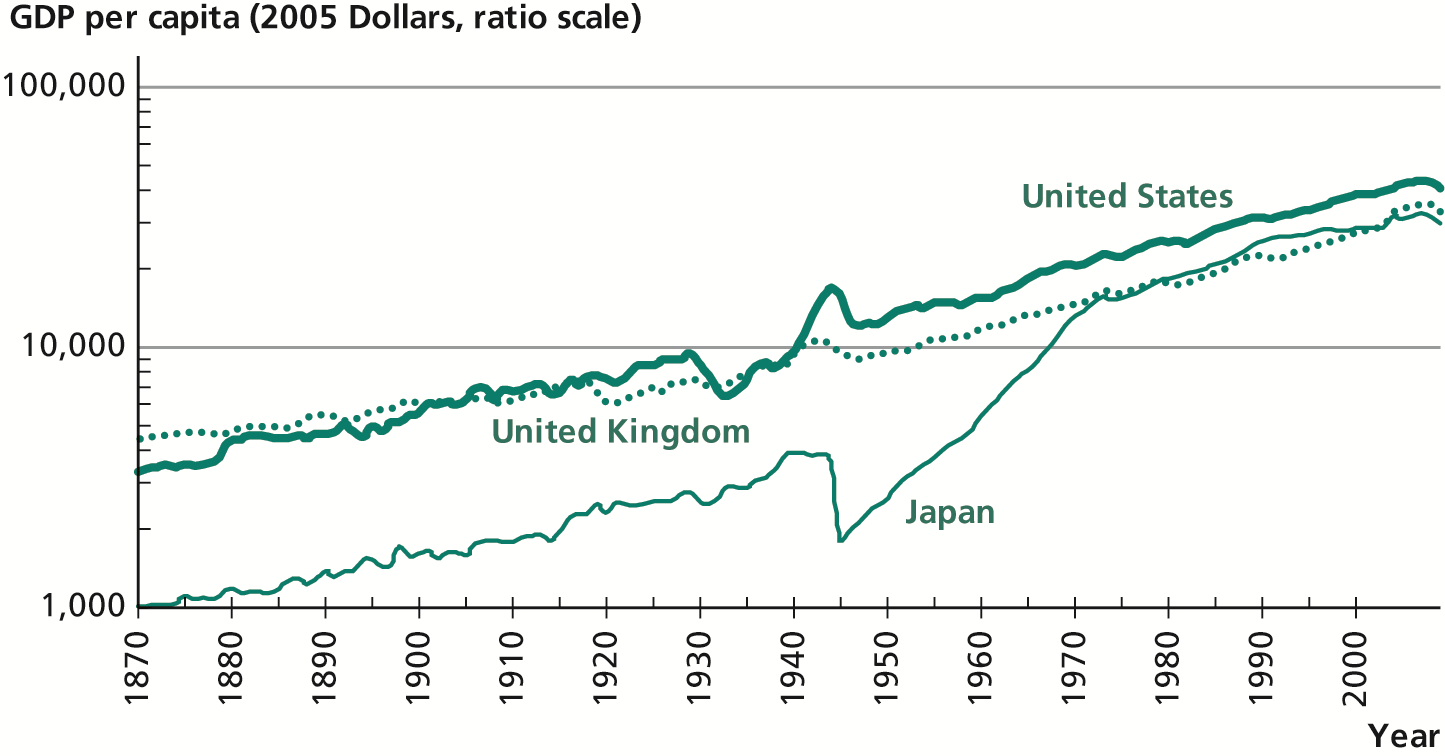
\includegraphics[width=.75\textwidth]{./img/1.5.png}
\end{center}
\end{frame}

\begin{frame}[label={sec:org8afce4d}]{}
\alert{Growth since 1970}
\begin{center}
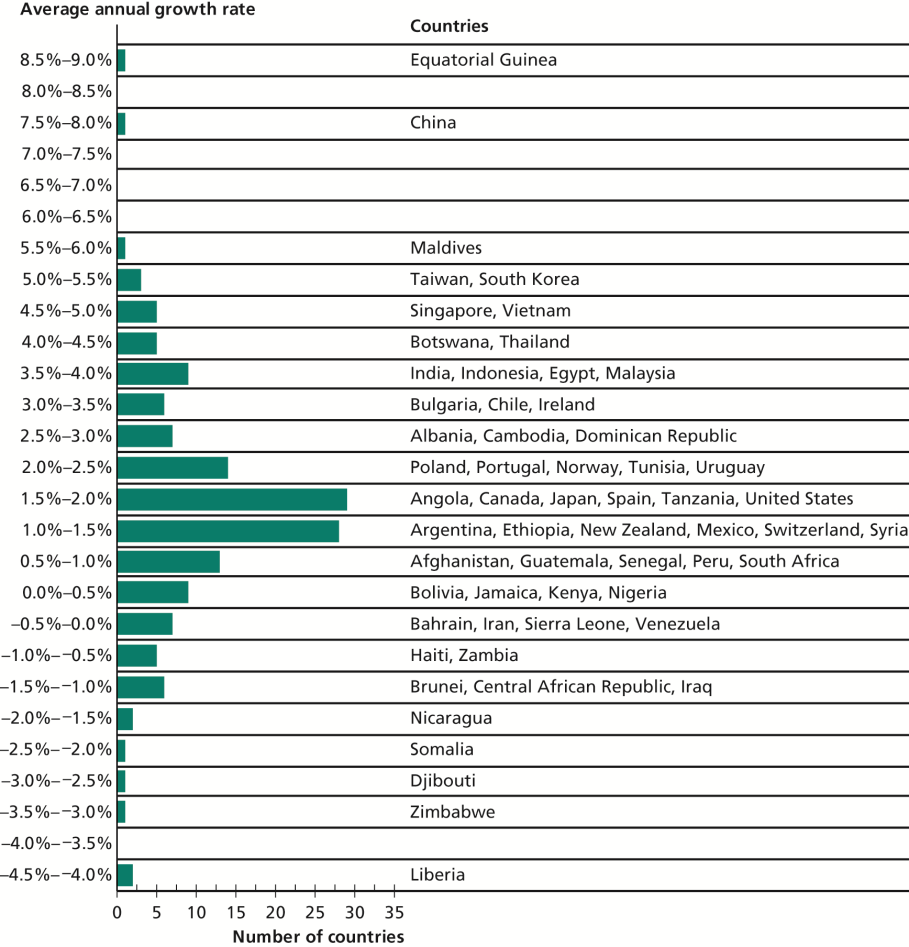
\includegraphics[width=.65\textwidth]{./img/1.6.png}
\end{center}
\end{frame}

\begin{frame}[label={sec:orgf9a1f46}]{}
\alert{Growth since 1820}
\begin{center}
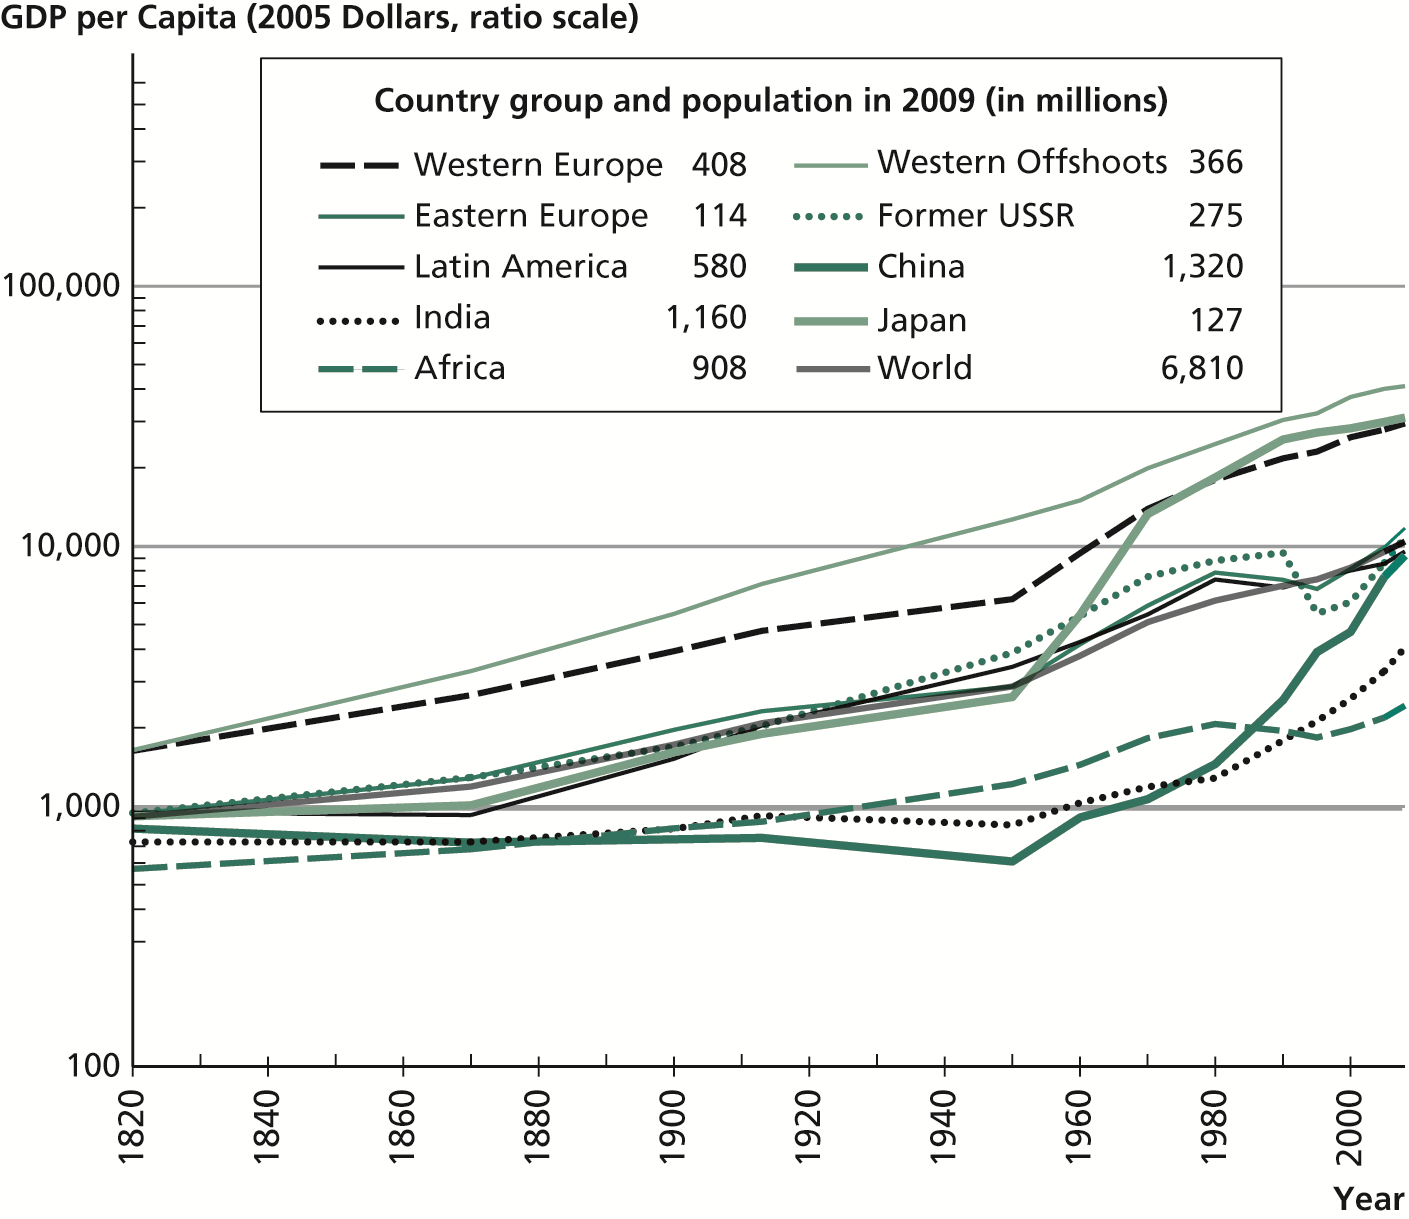
\includegraphics[width=.75\textwidth]{./img/1.7.png}
\end{center}
\end{frame}

\begin{frame}[label={sec:org457bfc1}]{}
\alert{Global growth facts}
\begin{itemize}
\item There is a large variation in growth rates
\item World income growth has accelerated over time
\item The gap between rich and poor countries is accelerating as well
\item Some countries seem to "transition" between growth rates
\end{itemize}
\end{frame}

\begin{frame}[label={sec:org54df4e2}]{}
\alert{Proximate vs fundamental causes}
\begin{itemize}
\item The purpose of this course is to investigate what \alert{causes} countries to have different growth rates
\item Proximate causes: Things that are immediately responsible for growth, e.g. factor accumulation, investment rates, technology, efficiency
\item Fundamental causes: Deeper causes of growth that determine proximate causes, e.g. culture, government, geography, institutions
\end{itemize}
\end{frame}

\begin{frame}[label={sec:org50d5b1c}]{}
\alert{Using data}
\begin{itemize}
\item Suppose we think that geography and fertility rates causally impact growth
\item How can we determine if this is true?
\item One possible solution is to plot the data and see if national income is correlated with our possible determinants
\end{itemize}
\end{frame}

\begin{frame}[label={sec:orga261f0f}]{}
\begin{center}
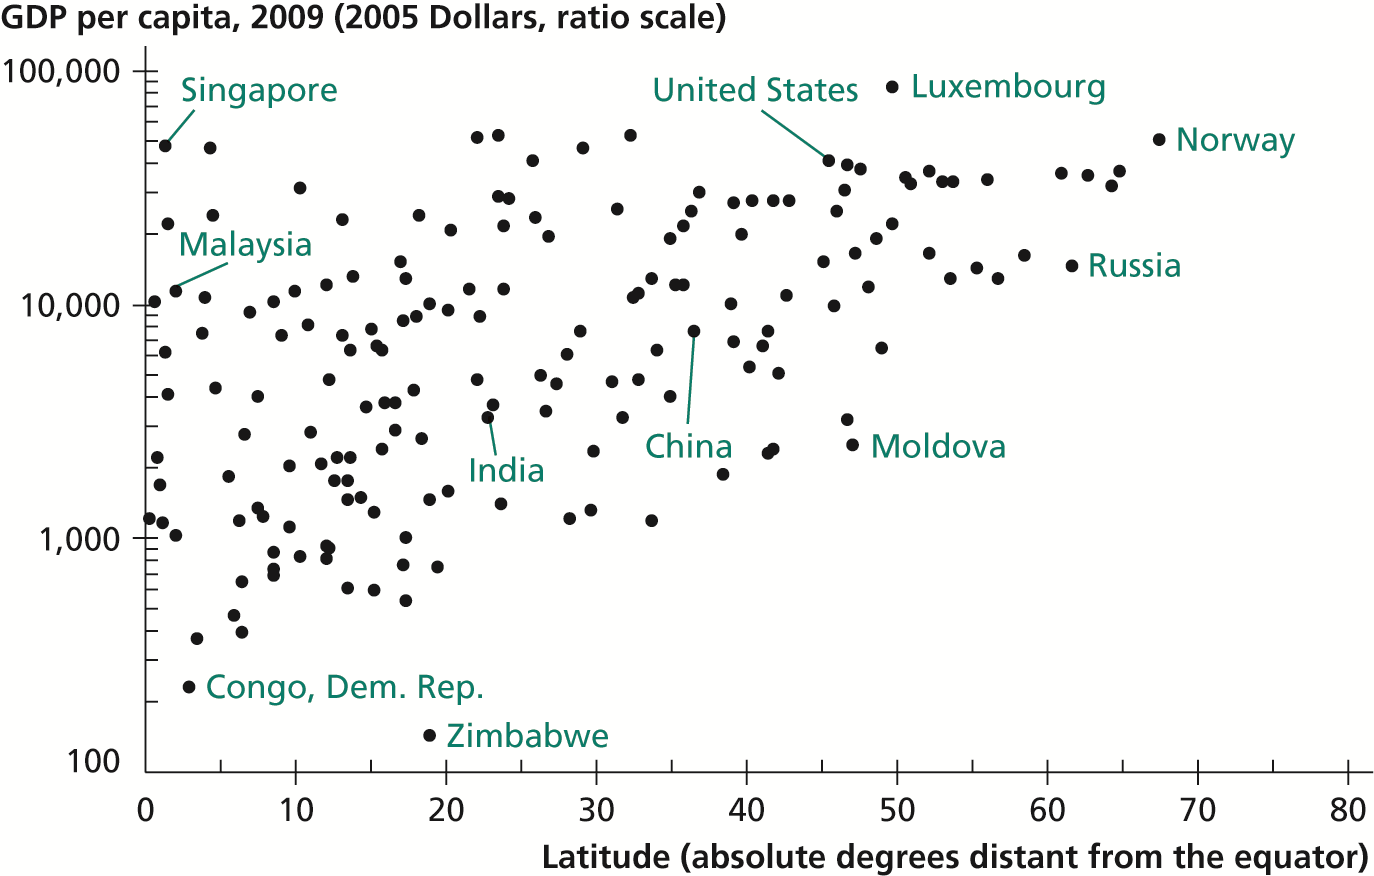
\includegraphics[width=.75\textwidth]{./img/2.3.png}
\end{center}
\end{frame}

\begin{frame}[label={sec:orga775876}]{}
\begin{center}
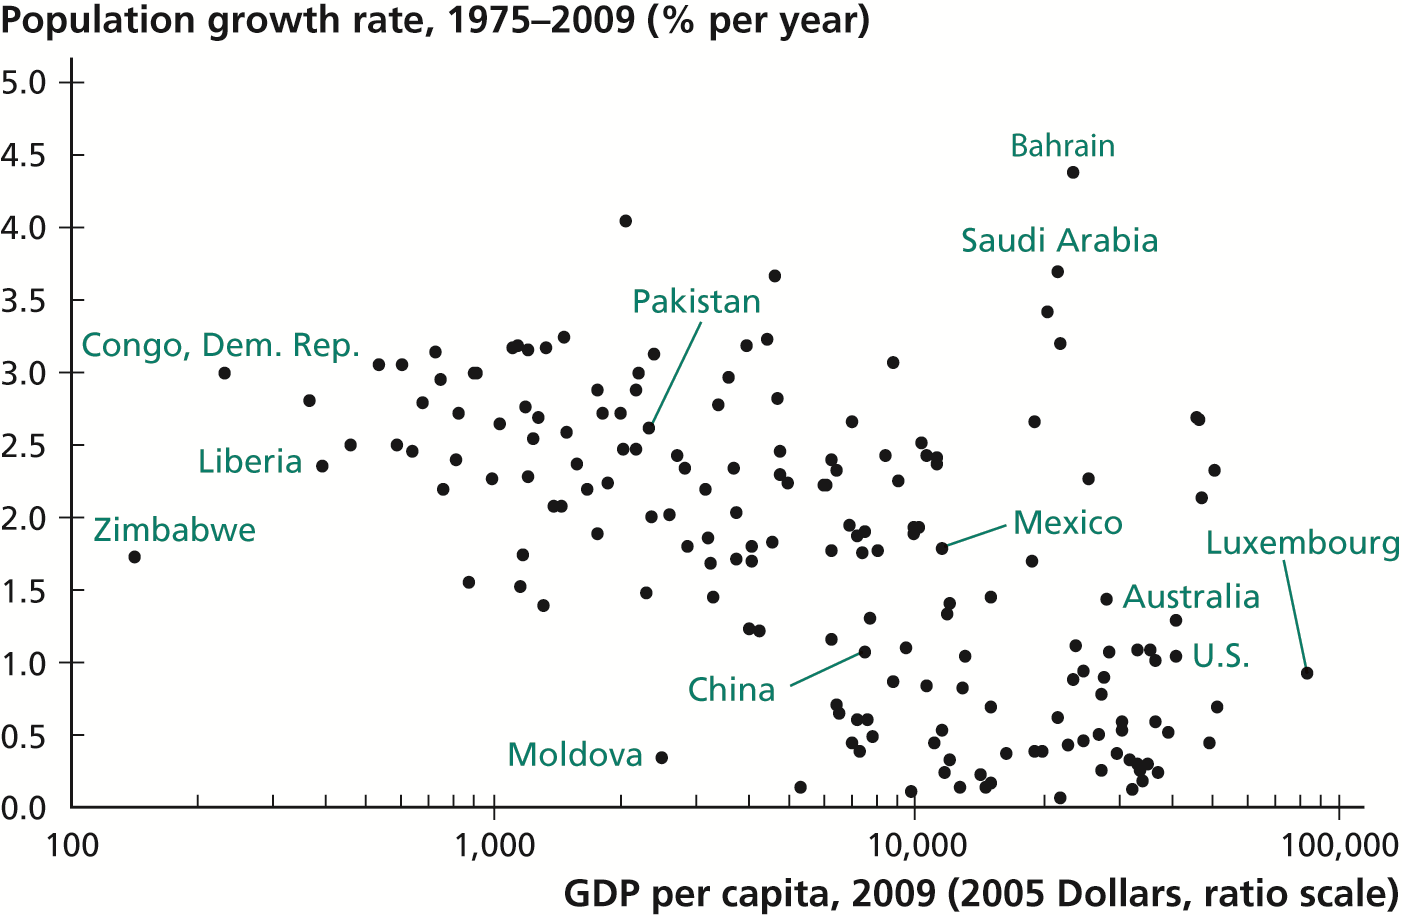
\includegraphics[width=.75\textwidth]{./img/2.4.png}
\end{center}
\end{frame}

\begin{frame}[label={sec:org7b674b1}]{}
\alert{Correlation and causality}
\begin{itemize}
\item Suppose we find that X and Y are correlated, and we suspect X causes Y. There are three possibilities:
\begin{enumerate}
\item X causes Y. If we change X, then we can expect Y to change as a result, just as we predicted.
\item Y causes X. "Reverse causality." If this is the case, then changing X will not influence Y.
\item No relationship between X and Y. "Omitted variable bias." A third variable causes both X and Y, but changing X or Y will not influence the other. Only the omitted variable is causally related.
\end{enumerate}
\end{itemize}
\end{frame}

\begin{frame}[label={sec:org73c2abf}]{}
\alert{Determining causality}
\begin{itemize}
\item Suppose we want to determine the causal effect of X on Y
\begin{itemize}
\item Many econometric tools can be used to help determine causality
\item Instrumental variables (IV): Find another variable Z that is correlated with X but not causally related to Y
\item Randomized control trials (RCT): Randomly assign "treatment" and "control" groups. Change X in treatment group, compare Y to control group.
\item It is difficult to randomize a "treatment" across countries, so IV is more common in growth economics. RCT more common in microeconomics, particularly in developing countries.
\end{itemize}
\end{itemize}
\end{frame}
\end{document}